%\VignetteEngine{Sweave} 
%\VignetteIndexEntry{Introduction to imputeTS}

\documentclass[a4paper]{report}
\usepackage[utf8]{inputenc}
\usepackage[T1]{fontenc}
\usepackage{RJournal}
\usepackage{amsmath,amssymb,array}
\usepackage{booktabs}
\RequirePackage[2014/12/31]{latexrelease}


\usepackage{Sweave}
\begin{document}
\input{Introduction-concordance}

%% do not edit, for illustration only
\sectionhead{Contributed research article}
\volume{XX}
\volnumber{YY}
\year{20ZZ}
\month{AAAA}

%% replace RJtemplate with your article
\begin{article}

%--------------------------------------

% !TeX root = RJwrapper.tex
\title{\pkg{imputeTS}: Time Series Missing Value Imputation in R}
\author{by Steffen Moritz and Thomas Bartz-Beielstein}

\maketitle



%================================================================================

\abstract{
The \pkg{imputeTS} package specializes on univariate time series imputation. It offers multiple state-of-the-art imputation algorithm implementations along with plotting functions for time series missing data statistics.
While imputation in general is a well-known problem and widely covered by R packages, finding packages able to fill missing values in univariate time series is more complicated. The reason for this lies in the fact, that most imputation algorithms rely on 
inter-attribute correlations, while univariate time series imputation instead needs to employ time dependencies. 
This paper provides an introduction to the \pkg{imputeTS} package and its provided algorithms and tools. Furthermore, it gives a short overview about univariate time series imputation in R.
}

%================================================================================

\section{Introduction}
\label{sec:Introduction}

In almost every domain from  industry \citep{billinton1996time} to  biology \citep{bar2003continuous}, finance \citep{taylor2007modelling} up to social science \citep{gottman1981time} different time series data are measured. While the recorded datasets itself may be different, one common problem are missing values. Many analysis methods require missing values to be replaced with reasonable values up-front. In statistics this process of replacing missing values is called \textit{imputation}.

\noindent\\
Time series imputation thereby is a special sub-field in the imputation research area. Most popular techniques like 
Multiple Imputation \citep{rubin1987multiple}, Expectation-Maximization  \citep{dempster1977maximum},  
Nearest Neighbor \citep{vacek1980examination} and Hot Deck \citep{ford1983overview} rely on 
 inter-attribute correlations to estimate values for the missing data. Since univariate time series do not possess 
more than one attribute, these algorithms cannot be applied directly. Effective univariate time series imputation 
algorithms instead need to employ the inter-time correlations. 

\noindent\\
On CRAN there are several packages 
solving the problem of imputation of multivariate data. Most popular and mature (among others) are \CRANpkg{AMELIA} \citep{AMELIA}, \CRANpkg{mice} \citep{mice}, \CRANpkg{VIM} \citep{VIM} and \CRANpkg{missMDA} \citep{missMDA}. However, since these packages are designed for multivariate data imputation only they do not work for univariate time series.

\noindent\\
At the moment \CRANpkg{imputeTS} \citep{imputeTS} is the only package on CRAN that is solely dedicated to univariate time series imputation and includes multiple algorithms.  Nevertheless, there are some other packages that include imputation functions as addition to their core package functionality. Most noteworthy being \CRANpkg{zoo} \citep{zoo} and \CRANpkg{forecast} \citep{forecast}. Both packages offer also some advanced time series imputation functions. The packages \CRANpkg{spacetime} \citep{spacetime}, \CRANpkg{timeSeries} \citep{timeSeries} and
\CRANpkg{xts} \citep{xts} should also be mentioned, since they contain some very simple but quick time series imputation methods. For a broader overview about available time series imputation packages in R see also \citep{Moritz15a}. In this  technical report we evaluate the performance of several univariate imputation functions in R on different time series. 

\noindent\\
This paper is structured as follows: Section~\nameref{sec:Overview imputeTS package} gives an overview, about all features and functions included in the \pkg{imputeTS} package. This is followed by~\nameref{sec:Usage examples} of the different provided functions. The paper ends with a~\nameref{sec:Conclusions} section.


%===============================================================================
\section{Overview \pkg{imputeTS} package}
\label{sec:Overview imputeTS package}

The \pkg{imputeTS} package can be found on CRAN and is an easy to use package that offers several utilities for \dfn{'univariate, equi-spaced, numeric time series'}. 

\noindent
Univariate means there is just one attribute that is observed over time. Which leads to a sequence of single observations $o_{1}$, $o_{2}$, $o_{3}$, ... $o_{n}$ at successive points $t_{1}$, $t_{2}$, $t_{3}$, ... $t_{n}$ in time. Equi-spaced means, that time increments between successive data points are equal $|t_{1} - t_{2}| = |t_{2} - t_{3}| = ... = |t_{n-1} - t_{n}|$. Numeric means that the observations are measurable quantities that can be described as a number.

\noindent
In the first part of this section, a general overview about all available functions and datasets is given. This is followed by more detailed overviews about the three areas covered by the package:  'Plots \& Statistics', 'Imputation' and 'Datasets'.
Information about how to apply these functions and tools can be found later in the ~\nameref{sec:Usage examples} section. 
\noindent\\

\subsection{General overview}
As can be seen in Table~\ref{tab:generaloverview}, beyond several imputation algorithm implementations the package also includes plotting functions and datasets. The imputation algorithms can be divided into rather simple but fast approaches like mean imputation and more advanced algorithms that need more computation time like kalman smoothing on a structural model. 

\begin{table}[h]
\centering
\begin{tabular}{@{}llll@{}}
\toprule
\textbf{Simple Imputation} & \textbf{Imputation} & \textbf{Plots \& Statistics} & \textbf{Datasets} \\ \midrule
na.locf                    & na.interpolation    & plotNA.distribution          & tsAirgap          \\
na.mean                    & na.kalman           & plotNA.distributionBar       & tsAirgapComplete  \\
na.random                  & na.ma               & plotNA.gapsize               & tsHeating             \\
na.replace                 & na.seadec           & plotNA.imputations           & tsHeatingComplete     \\
na.remove                  & na.seasplit         & statsNA                      & tsNH4         \\
                           &                     &                              & tsNH4Complete \\ \bottomrule
\end{tabular}
\caption{General Overview imputeTS package}
\label{tab:generaloverview}
\end{table}

\noindent
As a whole, the package aims to support the user in the complete process of replacing missing values in time series. This process starts with analyzing the distribution of the missing values using the \code{statsNA} function and the plots of  \code{plotNA.distribution}, \code{plotNA.distributionBar}, \code{plotNA.gapsize}. In the next step the actual imputation can take place with one of the several algorithm options. Finally, the imputation results can be visualized with the \code{plotNA.imputations} function. Additionally, the package contains three datasets, each in a version with and without missing values, that can be used to test imputation algorithms.
\noindent \\

\subsection{Plots \& Statistics functions}
An overview about the available plots and statistics functions can be found in Table~\ref{tab:overviewstatistics}. To get a good impression what the plots look like section ~\nameref{sec:Usage examples} is recommended. 

\begin{table}[h]
\centering
\begin{tabular}{@{}ll@{}}
\toprule
\textbf{Function}      & \textbf{Description}                               \\ \midrule
plotNA.distribution    & Visualize Distribution of Missing Values           \\
plotNA.distributionBar & Visualize Distribution of Missing Values (Barplot) \\
plotNA.gapsize         & Visualize Distribution of NA gap sizes              \\
plotNA.imputations     & Visualize Imputed Values                           \\
statsNA                & Print Statistics about the Missing Data            \\ \bottomrule
\end{tabular}
\caption{Overview Plots \& Statistics}
\label{tab:overviewstatistics}
\end{table}

\noindent
The \code{statsNA} function calculates several missing data statistics of the input data. This includes overall percentage of missing values, absolute amount of missing values, amount of missing value in different sections of the data, longest series of consecutive NAs and occurrence of consecutive NAs.
The \code{plotNA.distribution} function visualizes the distribution of NAs in a time series. This is done using a standard time series plot, in which areas with missing data are colored red. This enables the user to see at first sight where in the series most of the missing values are located. The \code{plotNA.distributionBar} function provides the same insights to users, but is designed for very large time series. This is necessary for time series with 1000 and more observations, where it is not possible to plot each observation as a single point.
The \code{plotNA.gapsize} function provides information about consecutive NAs by showing the most common NA gap sizes in the time series. The \code{plotNA.imputations} function is designated for visual inspection of the results after applying an imputation algorithm. Therefore, newly imputed observations are shown in a different color than the rest of the series.
\noindent \\

\subsection{Imputation functions}
An overview about all available imputation algorithms can be found in Table~\ref{tab:overviewimputation}. Even if these functions are really easy applicable, some examples can be found later in section~\nameref{sec:Usage examples}.
More detailed information about the theoretical background of the algorithms can be found in the \pkg{imputeTS} manual \citep{imputeTSmanual}.

\begin{table}[h]
\centering
\begin{tabular}{@{}lll@{}}
\toprule
\textbf{Function} & \textbf{Option} & \textbf{Description}                                            \\ \midrule
na.interpolation  &                 &                                                                 \\
                  & linear          & Imputation by Linear Interpolation                              \\
                  & spline          & Imputation by Spline Interpolation                              \\
                  & stine           & Imputation by Stineman Interpolation                            \\
na.kalman         &                 &                                                                 \\
                  & StructTS        & Imputation by Structural Model \& Kalman Smoothing              \\
                  & auto.arima      & Imputation by ARIMA State Space Representation \& Kalman Sm.    \\
na.locf           &                 &                                                                 \\
                  & locf            & Imputation by Last Observation Carried Forward                  \\
                  & nocb            & Imputation by Next Observation Carried Backward                 \\
na.ma             &                 &                                                                 \\
                  & simple          & Missing Value Imputation by Simple Moving Average               \\
                  & linear          & Missing Value Imputation by Linear Weighted Moving Average      \\
                  & exponential     & Missing Value Imputation by Exponential Weighted Moving Average \\
na.mean           &                 &                                                                 \\
                  & mean            & MissingValue Imputation by Mean Value                           \\
                  & median          & Missing Value Imputation by Median Value                        \\
                  & mode            & Missing Value Imputation by Mode Value                          \\
na.random         &                 & Missing Value Imputation by Random Sample                       \\
na.replace        &                 & Replace Missing Values by a Defined Value                       \\ \midrule
na.seadec         &                 & Seasonally Decomposed Missing Value Imputation                  \\
na.seasplit       &                 & Seasonally Splitted Missing Value Imputation                    \\ \midrule
na.remove         &                 & Remove Missing Values                                           \\ \bottomrule
\end{tabular}
\caption{Overview Imputation Algorithms}
\label{tab:overviewimputation}
\end{table}

\noindent
For convenience similar algorithms are available under one function name as parameter option.  For example linear, spline and stineman interpolation are all included in the 
\code{na.interpolation} function. The \code{na.mean}, \code{na.locf}, \code{na.replace}, \code{na.random} functions are all simple and fast. In comparison, \code{na.interpolation},
\code{na.kalman}, \code{na.ma}, \code{na.seasplit}, \code{na.seadec} are more advanced algorithms that need more computation time. The \code{na.remove} function is a special case, since it only deletes all missing values.
Thus, it is not really an imputation function. It should be handled with care since removing observations may corrupt the time information of the series. The \code{na.seasplit} and \code{na.seadec} functions are as well exceptions. These perform seasonal split / decomposition operations as a preprocessing step. For the imputation itself, one out of the other imputation algorithms 
can be used (which one can be set as option). Looking at all available imputation methods, no single overall best method can be pointed out. Imputation performance is always very dependent on the characteristics of the input time series. Even imputation with mean values can sometimes be an appropriate method. For time series with a strong seasonality usually \code{na.kalman} and \code{na.seadec} / \code{na.seasplit} perform best. In general, for most time series one algorithm out of \code{na.kalman}, \code{na.interpolation} and \code{na.seadec} will yield the best results. Meanwhile, \code{na.random}, \code{na.mean}, \code{na.locf} will be at the lower end accuracy wise for the majority of input time series.
\noindent\\

\subsection{Datasets}
\label{subsec:Datasets}
As can be seen in Table~\ref{tab:overviewdatasets}, all three datasets are available in a version with missing data and in a complete version. The provided time series are designated as benchmark datasets for univariate time series imputation. They shall enable users to quickly compare and test imputation algorithms. Without these datasets the process of testing time series imputation algorithms would require to manually delete certain observations. The benchmark data simplifies this: imputation algorithms can directly be applied to the dataset versions with missing values, which then can be compared to the complete dataset versions afterwards. Since the time series are specified, researchers can use these to compare their algorithms against each other.

\noindent\\
Reached RMSE or MAPE values on these datasets are easily understandable results to quote and compare against. Nevertheless, comparing algorithms using these fixed datasets can only be a first indicator of how well algorithms perform in general.  Especially for the very short \code{tsAirgap} series (with just 13 NA values) random lucky guesses can considerably influence the results. A complete benchmark would include: 'Different missing data percentages', 'Different datasets', 'Different random seeds for missing data simulation'.

\noindent\\
Overall there is a relatively small time series provided in \code{tsAirgap}, a medium one in \code{tsNH4} and a large time series in \code{tsHeating}. The \code{tsHeating} and \code{tsNH4} are both sensor data, while \code{tsAirgap} is count data.



\begin{table}[h]
\centering
\begin{tabular}{@{}ll@{}}
\toprule
\textbf{Dataset}  & \textbf{Description}                                               \\ \midrule
tsAirgap          & Time series of monthly airline passengers (with NAs)               \\
tsAirgapComplete  & Time series of monthly airline passengers (complete)               \\
tsHeating         & Time series of a heating systems' supply temperature (with NAs)     \\
tsHeatingComplete & Time series of a heating systems' supply temperature (complete)     \\
tsNH4             & Time series of NH4 concentration in a waste-water system (with NAs) \\
tsNH4Complete     & Time series of NH4 concentration in a waste-water system (complete) \\ \bottomrule
\end{tabular}
\caption{Overview Datasets}
\label{tab:overviewdatasets}
\end{table}

\noindent
\strong{tsAirgap}
\noindent\\
The \code{tsAirgap} time series has 144 rows and the incomplete version includes 14 NA values. It represents the monthly totals of international airline passengers from 1949 to 1960.
The time series originates from  \cite{Box76a} and is a commonly used example in time series analysis literature. Originally known as 'AirPassengers' or 'airpass' this version is renamed to 'tsAirgap' in order improve differentiation from the complete series (gap signifies that NAs were introduced). The characteristics (strong trend, strong seasonal behavior) make the \code{tsAirgap} series a great example for time series imputation.

\noindent
As already mentioned in order to use this series for comparing imputation algorithm results, there are two time series provided. One series without missing values (\code{tsAirgapComplete}), which can be used as ground truth. Another series with NAs, on which the imputation algorithms can be applied (\code{tsAirgap}). While the missing data for \code{tsNH4} and \code{tsHeating} were each introduced according to patterns observed in very similar time series from the same source, the missing observations in \code{tsAirgap} were created based on general missing data patterns.


\noindent\\
\strong{tsNH4}
\noindent\\
The \code{tsNH4} time series has 4552 rows and the incomplete version includes 883 NA values.  It represents  the NH4 concentration in a waste-water system measured from 30.11.2010 - 16:10 to 01.01.2011 - 6:40 in 10 minute steps.
The time series is derived from the dataset of the Genetic and Evolutionary Computation Conference (GECCO) Industrial Challenge 2014~\footnote{\url{http://www.spotseven.de/gecco-challenge/gecco-challenge-2014/}}.

\noindent
As already mentioned in order to use this series for comparing imputation algorithm results, there are two time series provided. One series without missing values (\code{tsNH4Complete}), which can be used as ground truth. Another series with NAs (\code{tsNH4}), on which the imputation algorithms can be applied. The pattern for the NA occurrence was derived from the same series / sensors, but from an earlier time interval. Thus, it is a very realistic missing data pattern. Beware, since the time series has a lot of observations, some of the more complex algorithms like \code{na.kalman} will need some time till they are finished.



\noindent\\
\strong{tsHeating}
\noindent\\
The \code{tsHeating} time series has 606837 rows and the incomplete version includes 57391 NA values.  It represents  a heating systems' supply temperature measured from 18.11.2013 - 05:12:00 to 13.01.2015 - 15:08:00 in 1 minute steps.
The time series originates from the GECCO Industrial Challenge 2015~\footnote{\url{http://www.spotseven.de/gecco-challenge/gecco-challenge-2015/}}. This was a challenge about 'Recovering missing information in heating system operating data'. Goal was to impute missing values in heating system sensor data as accurate as possible.

\noindent
As already mentioned in order to use this series for comparing imputation algorithm results, there are two time series provided. One series without missing values (\code{tsHeatingComplete}), which can be used as ground truth. Another series with NAs (\code{tsHeating}), on which the imputation algorithms can be applied. The NAs thereby were inserted according to patterns found in similar time series. According to patterns found / occurring in other heating systems. Beware, since it is a very large time series, some of the more complex algorithms like \code{na.kalman} may need up to several days to complete on standard hardware.


%================================================================================
\section{Usage examples}
\label{sec:Usage examples}

To start working with the \pkg{imputeTS} package, install either the stable version from CRAN or the development version from GitHub (\url{https://github.com/SteffenMoritz/imputeTS}). The stable version from CRAN is hereby recommended.

\subsection{Imputation algorithms}
All imputation algorithms are used the same way. Input has to be either a numeric time series or a numeric vector. As output, a version of the input data with all missing values replaced by imputed values is returned.
Here is a small example, to show how to use the imputation algorithms.
(all imputation functions start with na.'algorithm name')\\\\
\noindent
For this we first need to create an example input series with missing data.

\begin{example}
# Create a short example time series with missing values
 x <- ts(c(1, 2, 3, 4, 5, 6, 7, 8, NA, NA, 11, 12))
\end{example}

\noindent\\
On this time series we can apply different imputation algorithms. We start with using \code{na.mean}, which substitutes the NAs with mean values.

\begin{example}
# Impute the missing values with na.mean
 na.mean(x)
\end{example}
[1]~~~~1.0~~~~2.0~~~~3.0~~~~4.0~~~~5.0~~~~6.0~~~~7.0~~~~8.0
\textbf{~~~~5.9~~~~5.9}~~~~11.0~~~~12.0


\noindent\\
Most of the functions also have additional options that provide further algorithms (of the same algorithm category). In the example below it can be seen that \code{na.mean} can also be called with \code{option="median"}, which substitutes the NAs with median values.

\begin{example}
# Impute the missing values with na.mean using option median
 na.mean(x, option="median")
\end{example}
 [1]~~~~1.0~~~~2.0~~~~3.0~~~~4.0~~~~5.0~~~~6.0~~~~7.0
 ~~~~8.0~~~~\textbf{5.5~~~~5.5}~~~~11.0~~~~12.0
 
\noindent\\
While \code{na.interpolation} and all other imputation functions are used the same way, the results produced may be different. As can be seen below, for this series linear interpolation gives more reasonable results.
 
 
\begin{example}
# Impute the missing values with na.interpolation
na.interpolation(x)
\end{example}
[1]~~~~1~~~~2~~~~3~~~~4~~~~5~~~~6~~~~7
 ~~~~8~~~~\textbf{9~~~~10}~~~~11~~~~12
 
 \noindent\\
For longer and more complex time series (with trend and seasonality) than in this example it is always a good idea to try \code{na.kalman} and \code{na.seadec}, since these functions very often produce the best results. These functions are called the same easy way as all other imputation functions. 

 \noindent
Here is a usage example for the \code{na.kalman} function applied on the \code{tsAirgap} (described in ~\ref{subsec:Datasets}) time series. As can be seen in Figure~\ref{fig:imputations2}, \code{na.kalman} provides really good results for this series, which contains a strong seasonality and a strong trend. 

\begin{example}
# Impute the missing values with na.kalman
# (tsAirgap is an example time series provided by the imputeTS package)
imp <- na.kalman(tsAirgap)

#Code for visualization
plotNA.imputations(tsAirgap, x.imp, tsAirgapComplete)
\end{example}


\begin{figure} [hfbt]
\centering
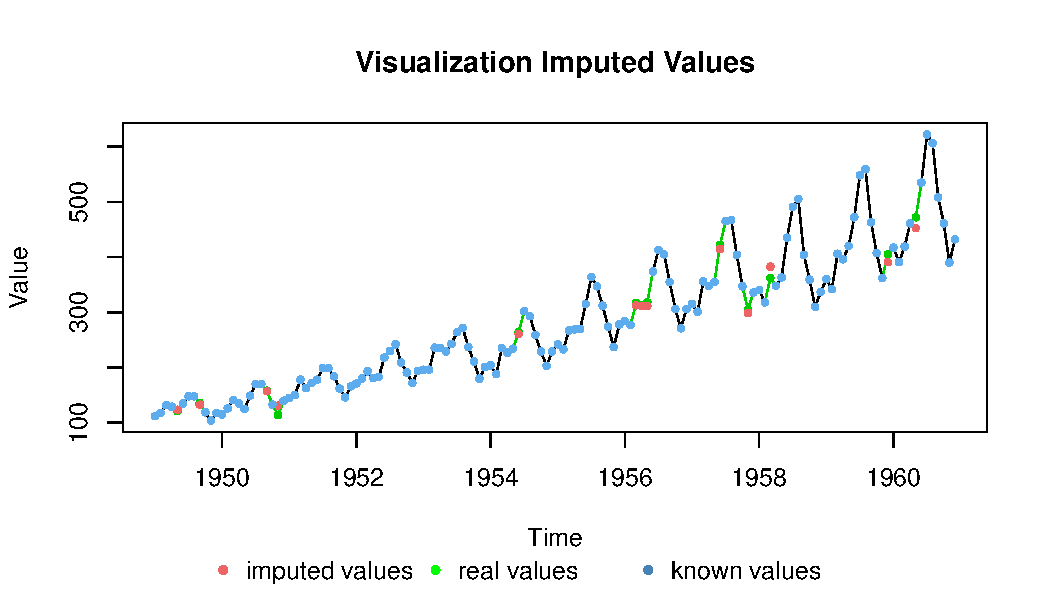
\includegraphics[width=5.7in]{Figures.d/imputations2.pdf}
\caption{Results of imputation with na.kalman compared to real values}
\label{fig:imputations2}
\end{figure}
\noindent

\subsection{plotNA.distribution}

This function visualizes the distribution of missing values within a time series. Therefore, the time series is plotted and whenever a value is NA the background is colored differently. This gives a nice overview, where in the time series most of the missing values occur. An example usage of the function can be seen below (for the plot see Figure~\ref{fig:distribution}).


\begin{example}
# Example Code 'plotNA.distribution'
# (tsAirgap is an example time series provided by the imputeTS package)

# Visualize the missing values in this time series
plotNA.distribution(tsAirgap)
\end{example}

\begin{figure} [hfbt]
\centering
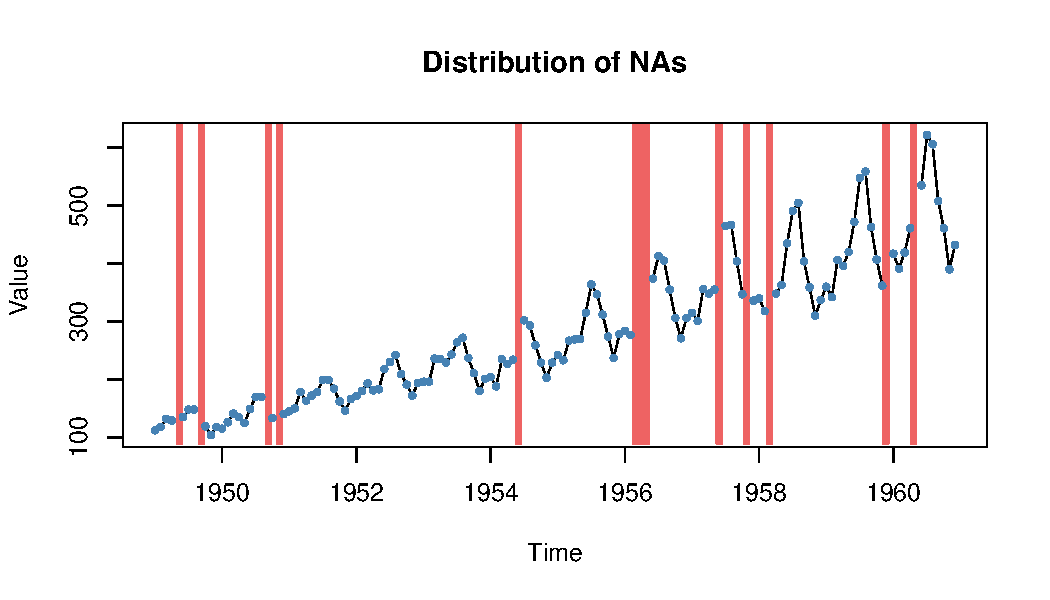
\includegraphics[width=5.7in]{Figures.d/distribution.pdf}
\caption{Example for plotNA.distribution}
\label{fig:distribution}
\end{figure}
\noindent
As can be seen in Figure~\ref{fig:distribution}, in areas with missing data the background is colored red. The whole plot is pretty much self-explanatory. The plotting function itself needs no further configuration parameters, nevertheless it allows passing through of plot parameters (via ...).
\noindent\\

\subsection{plotNA.distributionBar}
This function also visualizes the distribution of missing values within a time series. This is done as a barplot, which is especially useful if the time series would otherwise be too large to be plotted. Multiple observations for time intervals are grouped together and represented as bars. For these intervals, information about the amount of missing values are shown. An example usage of the function can be seen below (for the plot see Figure~\ref{fig:distributionBar}).

\begin{example}
# Example Code 'plotNA.distributionBar'
# (tsHeating is an example time series provided by the imputeTS package)

# Visualize the missing values in this time series
plotNA.distributionBar(tsHeating, breaks = 20)

\end{example}

\begin{figure} [hfbt]
\centering
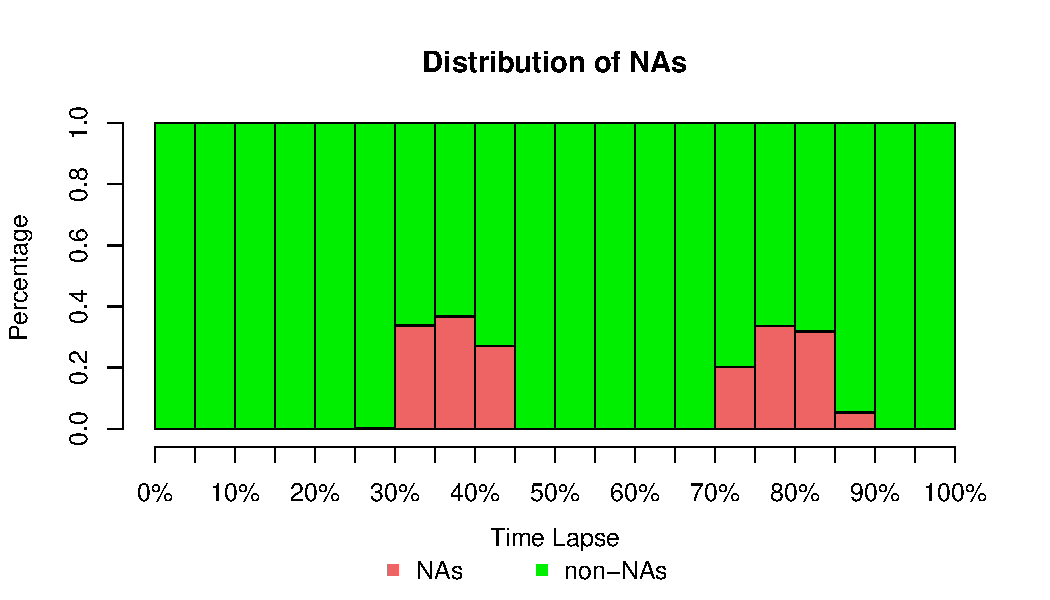
\includegraphics[width=5.7in]{Figures.d/distributionbar.pdf}
\caption{Example for plotNA.distributionBar}
\label{fig:distributionBar}
\end{figure}
\noindent\\
As can be seen in the x-axis of Figure~\ref{fig:distributionBar}, the \code{tsHeating} series is with over 600.000 observations a very large time series. While the missing values in the \code{tsAirgap} series (144 observations) can be visualized with \code{plotNA.distribution} like in Figure~\ref{fig:distribution}, this would for sure not work out for \code{tsHeating}. There just isn't enough space for 600.000 single consecutive observations/points in the plotting area. The \code{plotNA.distributionBar} function solves this problem. Multiple observations are grouped together in intervals. The 'breaks' parameter in the example defines that there should be 20 intervals used. This means every interval in Figure~\ref{fig:distributionBar} represents approximately 30.000 observations. The first five intervals are completely green, which means there are no missing values present. This means from observation 1 up to observation 150.000 there are no missing values in the data. In the middle and at the end of the series there are several intervals each having around 40\% of missing data. This means in these intervals 12.000 out of 30.000 observation are NA. All in all, the plot is able to give a nice  but rough overview about the NA distribution in very large time series. 
\noindent\\

\subsection{plotNA.gapsize}
This plotting function can be used to visualize how often different NA gaps (NAs in a row) occur in a time series. The function shows this information as a ranking. This ranking can be ordered by total NAs gap sizes account for (number occurrence gap size * gap length) or just by the number of occurrences of gap sizes. In the end the results can be read like this: In time series x, 3 NAs in a row occur most often with 20 occurrences, 6 NAs in a row occur 2nd most with 5 occurrences, 2 NAs in a row occur 3rd most with 3 occurrences.
An example usage of the function can be seen below(for the plot see Figure~\ref{fig:gapsize}).

\begin{example}

# Example Code 'plotNA.gapsize'
# (tsNH4 is an example time series provided by the imputeTS package)

# Visualize the top gap sizes / NAs in a row
plotNA.gapsize(tsNH4)

\end{example}

\begin{figure} [hfbt]
\centering
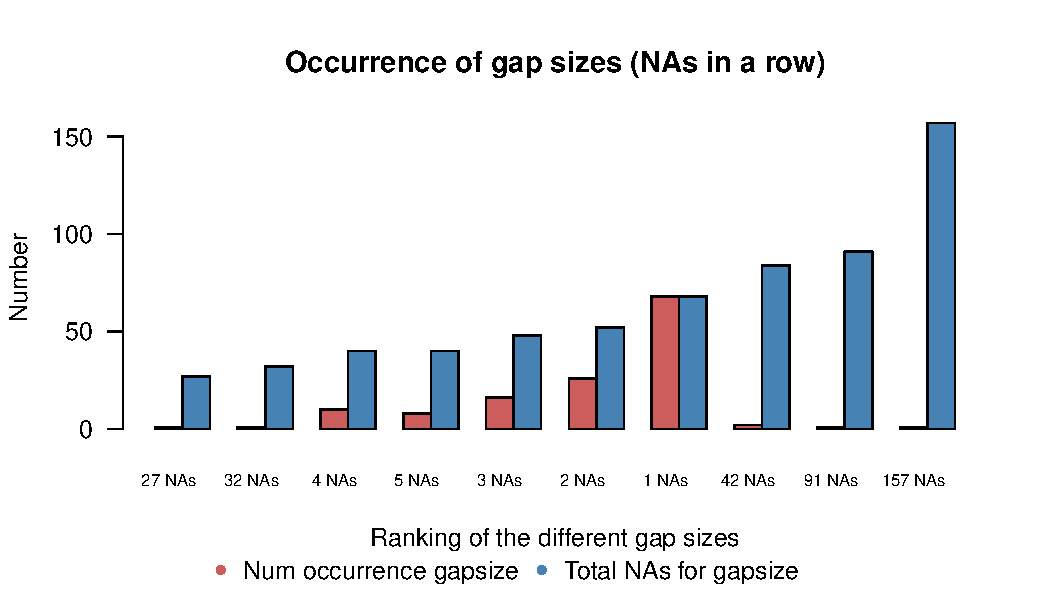
\includegraphics[width=5.7in]{Figures.d/gapsize.pdf}
\caption{Example for printNA.gapsize}
\label{fig:gapsize}
\end{figure}
 
 \noindent
The example plot (Figure~\ref{fig:gapsize}) reads the following: In the time series \code{tsNH4} gap size 157 occurs just 1 time, but makes up for most NAs of all gap sizes (157 NAs). A gap size of 91 (91 NAs in a row) also occurs just once, but makes up for 2nd most NAs (91 NAs). A gap size of 42 occurs two times in the time series, which leads to 3rd most overall (84 NAs). A gap size of one (no other NAs before or behind the NA) occurs 68 times, which makes this 4th in overall NAs (68 NAs). 
\noindent\\

\subsection{plotNA.imputations}
This plot can be used, to visualize the imputed values for a time series. Therefore, the imputed values (filled NA gaps) are shown in a different color than the other values. The function is used as below and Figure~\ref{fig:imputations} shows the output.

\begin{example}

# Example Code 'plotNA.imputations'
# (tsAirgap is an example time series provided by the imputeTS package)

# Step 1: Perform imputation for x using na.mean
tsAirgap.imp <- na.mean(tsAirgap)

# Step 2: Visualize the imputed values in the time series
plotNA.imputations(tsAirgap, tsAirgap.imp)


\end{example}

\noindent
The visual inspection of Figure~\ref{fig:imputations} indicates, that the imputed values (red) do not fit very well in the \code{tsAirgap} series. This is caused by \code{na.mean} being used for imputation of a series with a strong trend. The plotting function enables users to quickly detect such problems in the imputation results. If the ground truth is known for the imputed values, this information can also be added to the plot. The plotting function itself needs no further configuration parameters. Nevertheless, it allows passing through of plot parameters (via ...).
\noindent\\
\begin{figure} [hfbt]
\centering
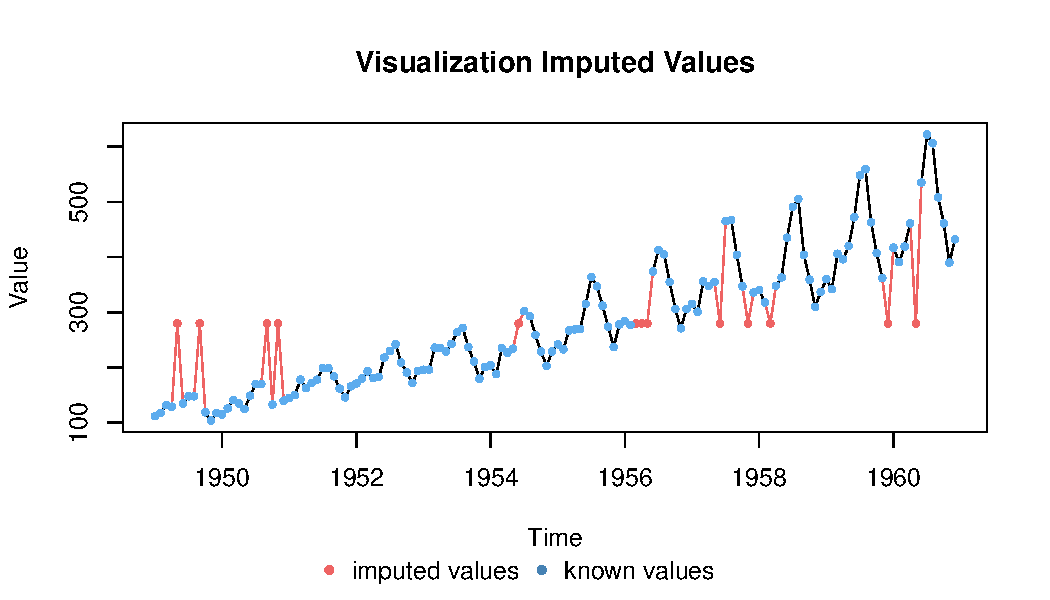
\includegraphics[width=5.7in]{Figures.d/imputations.pdf}
\caption{Example for printNA.imputations}
\label{fig:imputations}
\end{figure}

\subsection{statsNA}
The \code{statsNA} function prints summary stats about the distribution of missing values in univariate time series. Here is a short explanation about the information it gives:

\begin{itemize}
  \item Length of time series\\
  Number of observations in the time series (including NAs)
  \item Number of Missing Values\\
  Number of missing values in the time series
  \item Percentage of Missing Values
  Percentage of missing values in the time series
   \item Stats for Bins\\
  Number/percentage of missing values for the split into bins
  \item Longest NA gap\\
  Longest series of consecutive missing values (NAs in a row) in the time  
  series  
   \item Most frequent gap size\\
  Most frequent occurring series of missing values in the time series
  \item Gap size accounting for most NAs\\
  he series of consecutive missing values that accounts for most missing
  values overall in the time series
   \item Overview NA series\\
  Overview about how often each series of consecutive missing values
   occurs. Series occurring 0 times are skipped  
\end{itemize}

\noindent
The function is used as below and Figure~\ref{fig:statsNA} shows the output.
\noindent\\

\begin{example}
# Example Code 'statsNA'
# (tsNH4 is an example time series provided by the imputeTS package)

# Print stats about the missing data
statsNA(tsNH4)
\end{example}

\begin{figure} [hfbt]
\centering
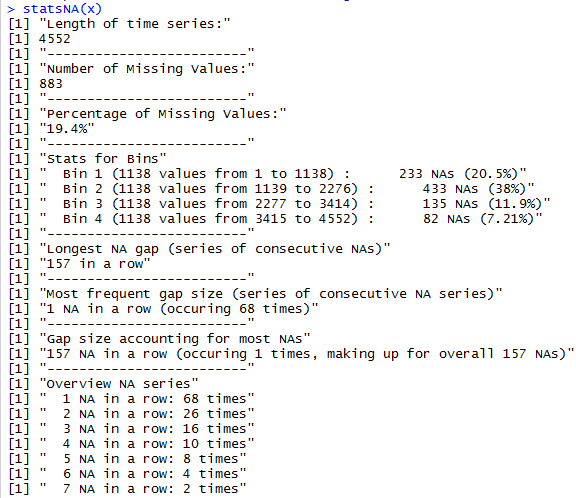
\includegraphics[width=5in]{Figures.d/statsna.png}
\caption{Excerpt of statsNA output}
\label{fig:statsNA}
\end{figure}

\subsection{Datasets}
Using the datasets is self-explanatory, after the package is loaded they are directly available and usable under their name. No call of data() is needed. For every dataset there is always a complete version (without NAs) and an incomplete version (containing NAs) available.

\begin{example}
# Example Code to use tsAirgap dataset
library("imputeTS")
tsAirgap
\end{example}

\begin{figure} [hfbt]
\centering
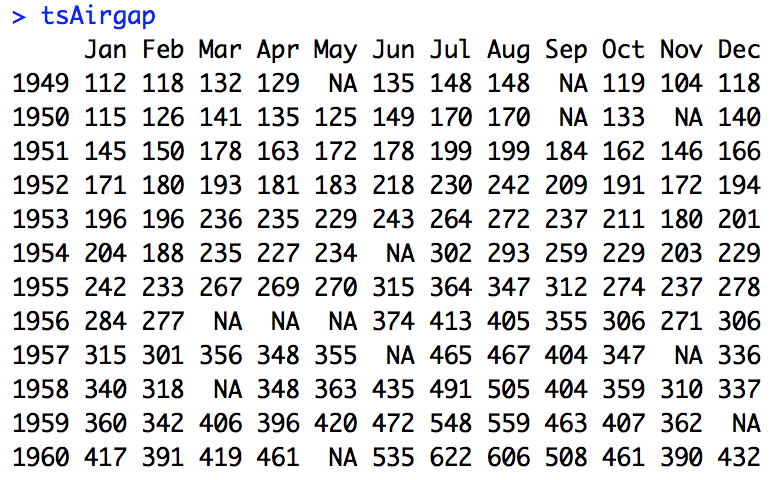
\includegraphics[width=4in]{Figures.d/tsairgap.png}
\caption{Example tsAirgap time series}
\label{fig:tsAirgap}
\end{figure}

%================================================================================
\section{Conclusions}
\label{sec:Conclusions}
Missing data is a very common problem for all kinds of data. However, in case of univariate time series most standard algorithms and existing functions within R packages cannot be applied.
\noindent\\
This paper presented the \pkg{imputeTS} package that provides a collection of  algorithms and tools especially tailored to this task. Using example time series, we illustrated the ease of use and the advantages of the provided functions. Simple algorithms as well as more complicated ones can be applied in the same simple and user-friendly manner.
\noindent\\\\
The functionality provided makes the \pkg{imputeTS} package a good choice for preprocessing of time series ahead of further analysis steps that require complete absence of missing values.
\noindent\\\\
Future research and development plans for forthcoming versions of the package include adding additional time series algorithm options to choose from. 


%================================================================================
\section{Acknowledgment}
\label{sec:Acknowlegment}
Parts of this work have been developed in the project '\textit{IMProvT: Intelligente Messverfahren zur Prozessoptimierung von Trinkwasserbereitstellung und -verteilung}' (reference number: 03ET1387A). Kindly supported by the Federal Ministry of Economic Affairs and Energy of the Federal Republic of Germany.

\begin{figure} [hfbt]
\centering

\includegraphics[width=2.5in]{Figures.d/sponsorlogo.jpg}
\label{fig:sponsor}
\end{figure}


%================================================================================

\begin{thebibliography}{21}
\providecommand{\natexlab}[1]{#1}
\providecommand{\url}[1]{\texttt{#1}}
\expandafter\ifx\csname urlstyle\endcsname\relax
  \providecommand{\doi}[1]{doi: #1}\else
  \providecommand{\doi}{doi: \begingroup \urlstyle{rm}\Url}\fi

\bibitem[Bar-Joseph et~al.(2003)Bar-Joseph, Gerber, Gifford, Jaakkola, and
  Simon]{bar2003continuous}
Z.~Bar-Joseph, G.~K. Gerber, D.~K. Gifford, T.~S. Jaakkola, and I.~Simon.
\newblock Continuous representations of time-series gene expression data.
\newblock \emph{Journal of Computational Biology}, 10\penalty0 (3-4):\penalty0
  341--356, 2003.

\bibitem[Billinton et~al.(1996)Billinton, Chen, and Ghajar]{billinton1996time}
R.~Billinton, H.~Chen, and R.~Ghajar.
\newblock Time-series models for reliability evaluation of power systems
  including wind energy.
\newblock \emph{Microelectronics Reliability}, 36\penalty0 (9):\penalty0
  1253--1261, 1996.

\bibitem[Box et~al.(2015)Box, Jenkins, Reinsel, and Ljung]{Box76a}
G.~E. Box, G.~M. Jenkins, G.~C. Reinsel, and G.~M. Ljung.
\newblock \emph{Time Series Analysis: Forecasting and Control}.
\newblock John Wiley \& Sons, 2015.

\bibitem[Dempster et~al.(1977)Dempster, Laird, and Rubin]{dempster1977maximum}
A.~P. Dempster, N.~M. Laird, and D.~B. Rubin.
\newblock Maximum likelihood from incomplete data via the {EM} algorithm.
\newblock \emph{Journal of the royal statistical society. Series B
  (methodological)}, pages 1--38, 1977.

\bibitem[Ford(1983)]{ford1983overview}
B.~L. Ford.
\newblock {An Overview of Hot-Deck Procedures}.
\newblock \emph{Incomplete data in sample surveys}, 2\penalty0 (Part
  IV):\penalty0 185--207, 1983.

\bibitem[Gottman(1981)]{gottman1981time}
J.~M. Gottman.
\newblock \emph{Time-series analysis: A comprehensive introduction for social
  scientists}, volume 400.
\newblock Cambridge University Press Cambridge, 1981.

\bibitem[Honaker et~al.(2011)Honaker, King, and Blackwell]{AMELIA}
J.~Honaker, G.~King, and M.~Blackwell.
\newblock {Amelia II: A Program for Missing Data}.
\newblock \emph{Journal of Statistical Software}, 45\penalty0 (7):\penalty0
  1--47, 2011.
\newblock URL \url{http://www.jstatsoft.org/v45/i07/}.

\bibitem[Hyndman(2016)]{forecast}
R.~J. Hyndman.
\newblock \emph{{forecast}: Forecasting functions for time series and linear
  models}, 2016.
\newblock URL \url{http://github.com/robjhyndman/forecast}.
\newblock R package version 7.3.

\bibitem[Josse and Husson(2016)]{missMDA}
J.~Josse and F.~Husson.
\newblock {missMDA: A Package for Handling Missing Values in Multivariate Data
  Analysis}.
\newblock \emph{Journal of Statistical Software}, 70\penalty0 (1):\penalty0
  1--31, 2016.
\newblock \doi{10.18637/jss.v070.i01}.

\bibitem[Kowarik and Templ(2016)]{VIM}
A.~Kowarik and M.~Templ.
\newblock Imputation with the {R} package {VIM}.
\newblock \emph{Journal of Statistical Software}, 74\penalty0 (7):\penalty0
  1--16, 2016.
\newblock \doi{10.18637/jss.v074.i07}.

\bibitem[Moritz(2016{\natexlab{a}})]{imputeTS}
S.~Moritz.
\newblock \emph{{imputeTS: Time Series Missing Value Imputation}},
  2016{\natexlab{a}}.
\newblock URL \url{http://CRAN.R-project.org/package=imputeTS}.
\newblock R package version 1.7.

\bibitem[Moritz(2016{\natexlab{b}})]{imputeTSmanual}
S.~Moritz.
\newblock \emph{package imputeTS}, 2016{\natexlab{b}}.
\newblock URL
  \url{http://cran.r-project.org/web/packages/imputeTS/imputeTS.pdf}.
\newblock R package version 1.7.

\bibitem[{Moritz} et~al.(2015){Moritz}, {Sard{\'a}}, {Bartz-Beielstein},
  {Zaefferer}, and {Stork}]{Moritz15a}
S.~{Moritz}, A.~{Sard{\'a}}, T.~{Bartz-Beielstein}, M.~{Zaefferer}, and
  J.~{Stork}.
\newblock {Comparison of different Methods for Univariate Time Series
  Imputation in R}.
\newblock \emph{ArXiv e-prints}, Oct. 2015.

\bibitem[Pebesma(2012)]{spacetime}
E.~Pebesma.
\newblock {spacetime: Spatio-Temporal Data in R}.
\newblock \emph{Journal of Statistical Software}, 51\penalty0 (7):\penalty0
  1--30, 2012.
\newblock URL \url{http://www.jstatsoft.org/v51/i07/}.

\bibitem[{Rmetrics Core Team} et~al.(2015){Rmetrics Core Team}, Wuertz, Setz,
  and Chalabi]{timeSeries}
{Rmetrics Core Team}, D.~Wuertz, T.~Setz, and Y.~Chalabi.
\newblock \emph{{timeSeries: Rmetrics - Financial Time Series Objects}}, 2015.
\newblock URL \url{https://CRAN.R-project.org/package=timeSeries}.
\newblock R package version 3022.101.2.

\bibitem[Rubin(1987)]{rubin1987multiple}
D.~B. Rubin.
\newblock \emph{Multiple imputation for nonresponse in surveys}.
\newblock New York: Wiley, 1987.

\bibitem[Ryan and Ulrich(2014)]{xts}
J.~A. Ryan and J.~M. Ulrich.
\newblock \emph{{xts: eXtensible Time Series}}, 2014.
\newblock URL \url{https://CRAN.R-project.org/package=xts}.
\newblock R package version 0.9-7.

\bibitem[Taylor(2007)]{taylor2007modelling}
S.~J. Taylor.
\newblock \emph{Modelling financial time series (second edition)}.
\newblock World Scientific Publishing, 2007.

\bibitem[Vacek and Ashikaga(1980)]{vacek1980examination}
P.~Vacek and T.~Ashikaga.
\newblock An examination of the nearest neighbor rule for imputing missing
  values.
\newblock \emph{Proc. Statist. Computing Sect., Amer. Statist. Ass}, pages
  326--331, 1980.

\bibitem[{van Buuren} and Groothuis-Oudshoorn(2011)]{mice}
S.~{van Buuren} and K.~Groothuis-Oudshoorn.
\newblock {mice: Multivariate Imputation by Chained Equations in R}.
\newblock \emph{Journal of Statistical Software}, 45\penalty0 (3):\penalty0
  1--67, 2011.
\newblock URL \url{http://www.jstatsoft.org/v45/i03/}.

\bibitem[Zeileis and Grothendieck(2005)]{zoo}
A.~Zeileis and G.~Grothendieck.
\newblock {zoo: S3 Infrastructure for Regular and Irregular Time Series}.
\newblock \emph{Journal of Statistical Software}, 14\penalty0 (6):\penalty0
  1--27, 2005.
\newblock URL \url{http://www.jstatsoft.org/v14/i06/}.

\end{thebibliography}



%================================================================================

\address{Steffen Moritz\\
  Cologne University of Applied Sciences\\
  Cologne, Germany\\}
\email{steffen.moritz10@gmail.com}


\address{Thomas Bartz-Beielstein\\
  Cologne University of Applied Sciences\\
  Cologne, Germany\\}
\email{bartz.beielstein@fh-koeln.de}


\end{article}

\end{document}
